\documentclass[border=4pt]{standalone}
\usepackage{tikz}
% Shared TikZ style: validated categorical palette (FP32 blue, FP16 orange, INT8 green, FP8 amber), light print surface.
\usetikzlibrary{arrows.meta,positioning,fit,backgrounds,calc,shapes.geometric}
\definecolor{fp32}{HTML}{2A78D6}
\definecolor{fp16}{HTML}{EB6834}
\definecolor{int8}{HTML}{1BAF7A}
\definecolor{fp8}{HTML}{EDA100}
\definecolor{ink}{HTML}{0B0B0B}
\definecolor{ink2}{HTML}{52514E}
\definecolor{muted}{HTML}{898781}
\definecolor{grid}{HTML}{E1E0D9}
\definecolor{surface}{HTML}{FCFCFB}
\definecolor{wash}{HTML}{F0EFEC}
\tikzset{
  font=\sffamily\small,
  box/.style={draw=muted, rounded corners=3pt, fill=surface, align=center, inner sep=4pt, text=ink},
  stage/.style={box, minimum height=1.0cm, text width=2.6cm},
  data/.style={box, fill=wash, draw=grid},
  result/.style={box, text width=2.9cm, minimum height=1.35cm},
  arrow/.style={-{Stealth[length=2.2mm]}, draw=ink2, line width=0.7pt},
  feedback/.style={arrow, dashed, draw=int8},
  tag/.style={font=\sffamily\scriptsize, text=ink2},
  group/.style={draw=grid, rounded corners=5pt, inner sep=6pt, line width=0.8pt},
}

\begin{document}
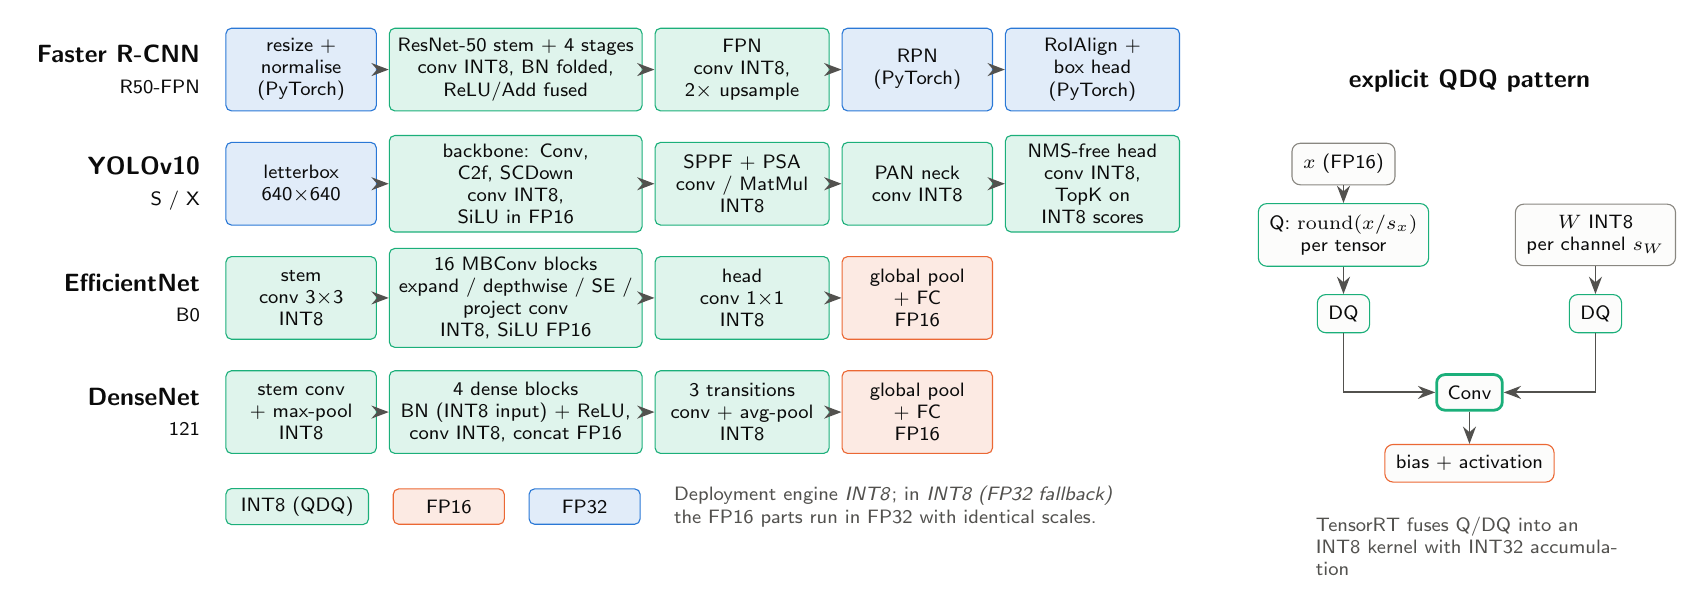
\begin{tikzpicture}[
  blk/.style={draw=#1, fill=#1!14, rounded corners=2pt, align=center, font=\sffamily\scriptsize, text=ink,
              minimum height=1.05cm, inner sep=3pt},
  lbl/.style={font=\sffamily\small\bfseries, text=ink, anchor=east, align=right},
  node distance=1.5mm]
% Row helper: label + chain of blocks
\node[lbl] at (-0.2,0) {Faster R-CNN\\\mdseries\scriptsize R50-FPN};
\node[blk=fp32, text width=1.7cm, anchor=west] (a1) at (0,0) {resize +\\normalise\\(PyTorch)};
\node[blk=int8, text width=3.0cm, right=of a1] (a2) {ResNet-50 stem + 4 stages\\conv INT8, BN folded,\\ReLU/Add fused};
\node[blk=int8, text width=2.0cm, right=of a2] (a3) {FPN\\conv INT8,\\2$\times$ upsample};
\node[blk=fp32, text width=1.7cm, right=of a3] (a4) {RPN\\(PyTorch)};
\node[blk=fp32, text width=2.0cm, right=of a4] (a5) {RoIAlign +\\box head\\(PyTorch)};

\node[lbl] at (-0.2,-1.45) {YOLOv10\\\mdseries\scriptsize S / X};
\node[blk=fp32, text width=1.7cm, anchor=west] (b1) at (0,-1.45) {letterbox\\640$\times$640};
\node[blk=int8, text width=3.0cm, right=of b1] (b2) {backbone: Conv, C2f, SCDown\\conv INT8,\\SiLU in FP16};
\node[blk=int8, text width=2.0cm, right=of b2] (b3) {SPPF + PSA\\conv / MatMul\\INT8};
\node[blk=int8, text width=1.7cm, right=of b3] (b4) {PAN neck\\conv INT8};
\node[blk=int8, text width=2.0cm, right=of b4] (b5) {NMS-free head\\conv INT8,\\TopK on INT8 scores};

\node[lbl] at (-0.2,-2.9) {EfficientNet\\\mdseries\scriptsize B0};
\node[blk=int8, text width=1.7cm, anchor=west] (c1) at (0,-2.9) {stem\\conv 3$\times$3\\INT8};
\node[blk=int8, text width=3.0cm, right=of c1] (c2) {16 MBConv blocks\\expand / depthwise / SE /\\project conv INT8, SiLU FP16};
\node[blk=int8, text width=2.0cm, right=of c2] (c3) {head\\conv 1$\times$1\\INT8};
\node[blk=fp16, text width=1.7cm, right=of c3] (c4) {global pool\\+ FC\\FP16};

\node[lbl] at (-0.2,-4.35) {DenseNet\\\mdseries\scriptsize 121};
\node[blk=int8, text width=1.7cm, anchor=west] (d1) at (0,-4.35) {stem conv\\+ max-pool\\INT8};
\node[blk=int8, text width=3.0cm, right=of d1] (d2) {4 dense blocks\\BN (INT8 input) + ReLU,\\conv INT8, concat FP16};
\node[blk=int8, text width=2.0cm, right=of d2] (d3) {3 transitions\\conv + avg-pool\\INT8};
\node[blk=fp16, text width=1.7cm, right=of d3] (d4) {global pool\\+ FC\\FP16};

\foreach \r in {a,b} {\foreach \i/\j in {1/2,2/3,3/4,4/5} {\draw[arrow] (\r\i) -- (\r\j);}}
\foreach \r in {c,d} {\foreach \i/\j in {1/2,2/3,3/4} {\draw[arrow] (\r\i) -- (\r\j);}}

% legend
\node[blk=int8, minimum height=0.45cm, text width=1.6cm, anchor=west] (l1) at (0,-5.55) {INT8 (QDQ)};
\node[blk=fp16, minimum height=0.45cm, text width=1.2cm, right=3mm of l1] (l2) {FP16};
\node[blk=fp32, minimum height=0.45cm, text width=1.2cm, right=3mm of l2] (l3) {FP32};
\node[tag, right=3mm of l3, align=left] {Deployment engine \emph{INT8}; in \emph{INT8 (FP32 fallback)}\\the FP16 parts run in FP32 with identical scales.};

% zoom: explicit quantization pattern
\begin{scope}[shift={(14.2,-1.2)}]
\node[font=\sffamily\small\bfseries, text=ink] at (1.6,1.05) {explicit QDQ pattern};
\node[box, font=\sffamily\scriptsize] (x) at (0,0) {$x$ (FP16)};
\node[box, draw=int8, font=\sffamily\scriptsize] (q) at (0,-0.9) {Q: $\mathrm{round}(x/s_x)$\\per tensor};
\node[box, draw=int8, font=\sffamily\scriptsize] (dq) at (0,-1.9) {DQ};
\node[box, font=\sffamily\scriptsize] (w) at (3.2,-0.9) {$W$ INT8\\per channel $s_W$};
\node[box, draw=int8, font=\sffamily\scriptsize] (dqw) at (3.2,-1.9) {DQ};
\node[box, draw=int8, line width=1pt, font=\sffamily\scriptsize] (conv) at (1.6,-2.9) {Conv};
\node[box, draw=fp16, font=\sffamily\scriptsize] (act) at (1.6,-3.8) {bias + activation};
\draw[arrow] (x) -- (q); \draw[arrow] (q) -- (dq); \draw[arrow] (w) -- (dqw);
\draw[arrow] (dq) |- (conv); \draw[arrow] (dqw) |- (conv); \draw[arrow] (conv) -- (act);
\node[tag, align=left, text width=3.9cm] at (1.6,-4.85) {TensorRT fuses Q/DQ into an INT8 kernel with INT32 accumulation};
\end{scope}
\end{tikzpicture}
\end{document}
